\documentclass[a4paper,11pt,leqno,notitlepage,onecolumn]{article}
%\documentclass[a4paper,11pt,leqno,notitlepage,twocolumn]{article}

\usepackage[latin1]{inputenc}
\usepackage{fontenc}
\usepackage{graphicx}
\usepackage[dvips]{hyperref}
\usepackage{subfigure}
\usepackage{setspace}
\doublespacing
\usepackage[a4paper]{geometry}
\geometry{top=1.2in, bottom=1.2in, left=1.2in, right=1.2in}
%\geometry{top=1in, bottom=1in, left=1in, right=1in}

\begin{document}
\title{PIX: PMaC's Efficient Binary Instrumentor for Linux on x86 Platforms}
\author{Michael Laurenzano, Mustafa M. Tikir, Laura Carrington, Allan Snavely\\
San Diego Supercomputer Center\\
9500 Gilman Drive, La Jolla, CA 92037\\
\it{\{michaell,mtikir,laurac,allans\}@sdsc.edu}}
\date{}
\maketitle

\begin{abstract}
\begin{it}

Binary instrumentation enables insertion of additional code into an
executable in order to observe or modify the behavior of application runs. 
There are two main approaches to binary instrumentation: static and dynamic
binary instrumentation. In this paper, we present PMaC's instrumentation toolkit (PIX), 
an efficient static  instrumentation toolkit for Linux on x86/x86\_64 platforms. PIX
is similar to the other toolkits in terms of how additional code is inserted. However, it uses whole function level
code relocation in order to remedy the difficulty created by the variable-length instruction set. Code relocation of this kind allows the
instrumentation tool to reorganize the application code in such a way that it
can use the fast  far-reaching constructs to transfer control
from the application to the instrumentation code rather than relying on multiple
jumps or interrupts for the transfer. Furthermore, the PIX API provides a means to
tool developers to insert lightweight hand-coded assembly
rather than relying solely on the insertion of entire instrumentation functions.
PIX also enables implementation of efficient instrumentation tools, 
with overheads  for basic block counting that are an
average of 2.1x less overhead imposed by Pin, 5.6x less overhead imposed by
DynamoRIO, 10.0x less overhead imposed by Valgrind, and XXX\% less overhead imposed by Dyninst.

\end{it}

\end{abstract}

\section{Introduction}

Binary instrumention is the act of inserting extra code into a compiled
application in order to observe or modify something about its behavior. The data
collected from binary instrumentation can be useful for guiding hardware and
system design decisions, program debugging, compiler correctness/optimization,
program debugging and security testing/verification.

There are two common approaches to binary instrumentation: static binary
instrumentation and dynamic binary instrumentation. Static binary
instrumentation toolkits have the advantage of usually being able to produce
more efficient instrumented code than comparable dynamic binary instrumentation toolkits
because static instrumentation introduces only the instrumentation code itsself into the run of the
application. Static binary instrumentation tools have some disadvantages,
however. It is not possible to instrument shared libraries or dyanamically
generated code with static binary instrumentation tools. They also provide less
flexibility to the tool developer, since any instrumentation code that is
inserted into the application will persist throughout the application run.
However, there are cases where efficiency is of enough importance to outweigh
these shortcomings in such a way that static binary instrumentation is the
desirable paradigm.

x86elfinstrumentor is a static binary instrumentation toolkit for Linux on
X86/X86\_64 platforms. The goal of x86elfinstrumentor is to provide the ability
to build instrumentation tools that produce very efficient instrumented
applications. We instrument the binary by placing an unconditional branch at each instrumentation
point that transfers control to instrumentation code. This instrumentation code saves the
program state, performs some functions that are determined by the particular instrumentation tool,
restores the program state, then returns control to the application.
A typical binary instrumentation tool on a platform with fixed-length instructions 
\cite{tikir2006pmac} accomplishes this initial control transfer by replacing a
single instruction at the instrumentation point with a branch that transfers
control to the instrumentation code. However when instructions are variable-length, as
is the case for X86/X86\_64, this is not always possible since the branch instruction can be larger than the
instruction at the instrumentation point. To address this, x86elfinstrumentor
relocates and reorganizes the code for each function to ensure that enough empty
space (in the form of \begin{it}nops\end{it}) is available to hold a full-length branch instruction at each
instrumentation point.

Instrumented code efficiency is accomplished in several ways. The cost of
instrumentation, tasks such as parsing, disassembly and code generation, is
taken prior to runtime rather than at runtime as is done by current state of the
art binary instrumentation tools for X86/X86\_64 \cite{luk2005pin,
nethercote2007valgrind, dynamorio}. We relocate the application's
functions, which affords us the opportunity to reorganize the code so that we
can use large yet efficient instructions to transfer control from the
application to the instrumentation code. We also use the concept of an
instrumentation snippet, a lightweight hand-written body of assembly code that can
be inserted into the application rather than inserting only heavyweight
functions to accomplish instrumentation tasks.

x86elfinstrumentor is open source and available to the public for download along with several
instrumentation tools at \url{http://blind-review-forbids-real-urls.com/}. These tools include a basic block
execution counter, a function execution counter, and a memory address stream collection tool.

The rest of the paper is organized as follows. Section
\ref{Section:Overview} descries the design and implementation of our static
instrumentation toolkit. Section \ref{Section:Challenges} discusses in greater detail
several aspects of the toolkit, including the function relocation mechanism and the
instrumentation snippet concept. Section \ref{Section:Tools} shows the details of
the instrumentation tools included in the package. Section \ref{Section:Results}
presents a comparison and discussion of the performance of x86elfinstrumentor relative
to other state of the art instrumentation toolkits. Section
\ref{Section:Future} discusses some ideas for the future of x86elfinstrumentor,
and Section \ref{Section:Conclusions} concludes.


\section{Overview}

Static binary instrumentation results in a modified executable 
 that can be run at a later time. When the instrumented executable is
run, the extra instrumentation code inserted by the instrumentation tool is run
in addition to the original code of the program. In order to insert additional code
and data, additional space must be allocated within the executable in a way that it
will, at load-time, be treated by the system in a manner appropriate to its
purpose. 

Most compilers produce an executable whose
structure is similar to that shown in Figure \ref{Figure:Executable}. By
convention, most executables use only two loadable segments and some of the Linux
implementations, such as FreeBSD, only allow two loadable segments. Thus it is
preferrable for us to incorparate instrumentation text and data into the
existing text and data segments of the application. The default in most
compilers is to place the text segment prior and adjacent to the data segment.
We therefore prepend the instrumentation text to the existing text
segment\footnote{The amount of space allocated prior to the text section is
controlled by the linker variable \_\_executable\_start. We have seen cases
where the system does not provide enough space prior to the text segment by
default, in which case we provide a set of tools that produces a modified linker
script that provides 128Mb of space.} and append the instrumentation data to the
data segment (as shown in Figure \ref{Figure:InstExecutable}). This
scheme has the added benefit of causing no immediate disturbance to the
addresses of the existing text and data segments of the program.

\begin{figure}[ht]
\centering
\caption[Optional caption for list of figures]{\subref{Figure:OrigExecutable} and \subref{Figure:InstExecutable} show the prepending
of instrumentation text to the existing text, and the prepending of instrumentation data to the existing data respectively.}
\subfigure[The two-segment structure of an unmodified ELF file.]{
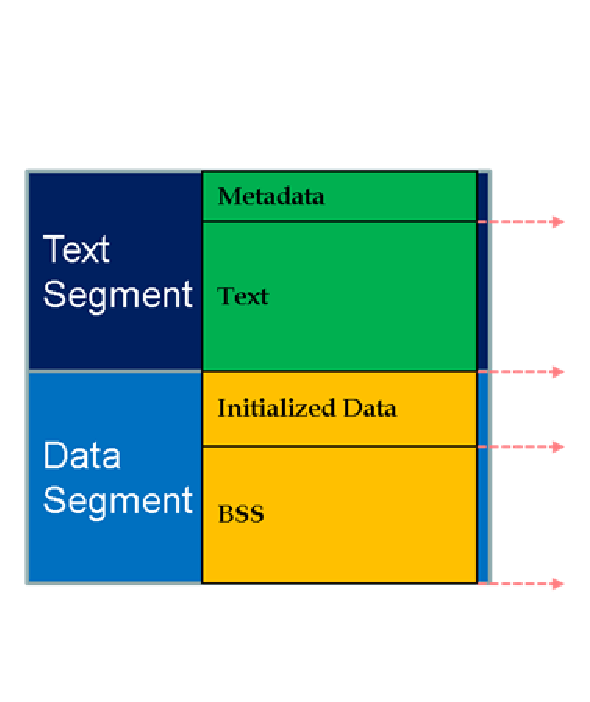
\includegraphics[scale=0.65]{executablep1.eps}
\label{Figure:OrigExecutable}
}
\subfigure[The two-segment structure of the ELF file once instrumentation code and data are inserted.]{
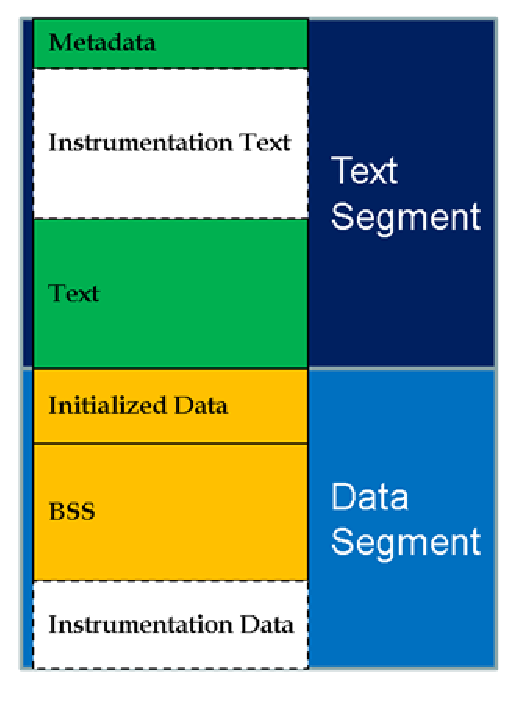
\includegraphics[scale=0.65]{executablep2.eps}
\label{Figure:InstExecutable}
}
\label{Figure:Executable}
\end{figure}

The instrumentation text contains several types of instrumentation code. The first
contains code that accomplishes the instrumentation task as well as some code to
accompany it. When control is transferred from the application to the
instrumentation code, it is necessary to maintain the machine state of
the application in order to preserve its original behavior. This machine state
can contain anything modified by the instrumentation code, but in practice is
usually limited to a relatively limited set of registers. The code snippet, called \textit{trampoline} [CITE Dyninst], 
saves any registers it intends to use, performs the instrumentation task, restores
any machine state after the instrumentation, executes the
original instructions that were displaced by the initial control transfer,
finally restoring control to the application. Since we are using an
unconditional branch instruction at the instrumentation point, at runtime the
instrumentation code has no information about where control was transferred from
(as might be the case if we used a more heavyweight call instruction). Hence
each instrumentation point uses its own trampoline so that the location of the
instrumentation point can be hard-coded into an unconditional branch instruction
at the end of the trampoline.

The instrumentation text also includes code to initialize data for use by the
instrumentation tool. Recall from Figure \ref{Figure:Executable} that the instrumentation
data was appended to the end of the application's data segment, after the
application's uninitialized data section  (BSS section). The initialized data and BSS
sections of the data segment are usually implemented by declaring the size of
the data segment in the executable to be smaller than the size of the data
segment in memory. According to the ELF[CITE] specification, the extra part of any
segment whose memory size is greater than its file size should be filled with
zeroes by the loader. Hence most programs just increase the size of the data
segment's size in memory by the size of the BSS section in order to get a large
area that is filled with zeroes and is reserved for uninitialized data. Since we
would like to use the area following the BSS section for (possibly initialized)
data for the instrumentation tool, we can either explicitly include the entire
segment's contents in the executable file or we can implicitly reserve this area
using the technique described above that is already in use by most programs.
Since the BSS section can be very large and explicit inclusion of its contents
would bloat the instrumented executable file unnecessarily, we use the implicit
technique to reserve this section for instrumentatoin data. We therefore
temporarily store the instrumentation data with the instrumentation text in the
executable, as well as some code to copy it to the appropriate location in the
data segment once the program starts.


\section{Efficiency of Instrumented Code}
\label{sec:Efficiency}

The goal of PEBIL is to provide a toolkit that enables the construction of
instrumentation tools that produce efficient instrumented executables.
Specifically PEBIL is designed to provide efficiency when there are a large
number of instrumentation points because it is these cases where instrumentation
has the largest overhead on application performance. Several techniques are
employed to produce efficient instrumented code. One such technique is the use
of fast constructs to get control to the instrumentation code, which requires
the application code to be relocated and transformed. PEBIL also allows the use
of lightweight instrumentation snippets that can be used in place of
instrumentation functions for simple instrumentation tasks.

\subsection{Code Relocation and Transformation}
\label{Subsection:Relocation}
The use of relocation at the function level in PEBIL stems from the fact that
instrumentation is being performed statically on a platform that uses a
variable-length instruction set. The presence of variable-length length
instructions means that it may not always be possible to instrument an arbitrary
point using traditional techniques due to the lack of space at the
instrumentation point for a jump instruction large enough to reach the
instrumentation code. A common strategy used by static instrumentation toolkits
on platforms with fixed-length instruction sets is to replace a single
instruction at the instrumentation point with a branch instruction that will
transfer control to the instrumentation code. This is fairly straightforward
because, by the definition of a fixed-length instruction set, the instruction
being replaced and the replacing jump instruction have the same length. In x86
platforms, a jump instruction that uses a 32-bit offset requires 5 bytes.
However, for some instrumentation points of interest there may not be enough
space to hold a 5 byte jump instruction because the instrumentation point itself
(which might be an instruction or a basic block) is smaller than 5 bytes. 

Figure \ref{fig:InstructionSizes} shows a breakdown of the sizes of instructions
for a set of the SPEC CPU2000 Integer benchmarks. This figure shows that for
these benchmarks, between 52\% and 74\% of instructions are smaller than 5
bytes. In fact an average of 64\% of instructions are smaller, which indicates
that the the generic technique of replacing an instruction with a branch to
instrumentation code cannot provide instrumentation to large portions of the application
code.

\begin{figure}[ht]
\centering
\label{fig:InstructionSizes}
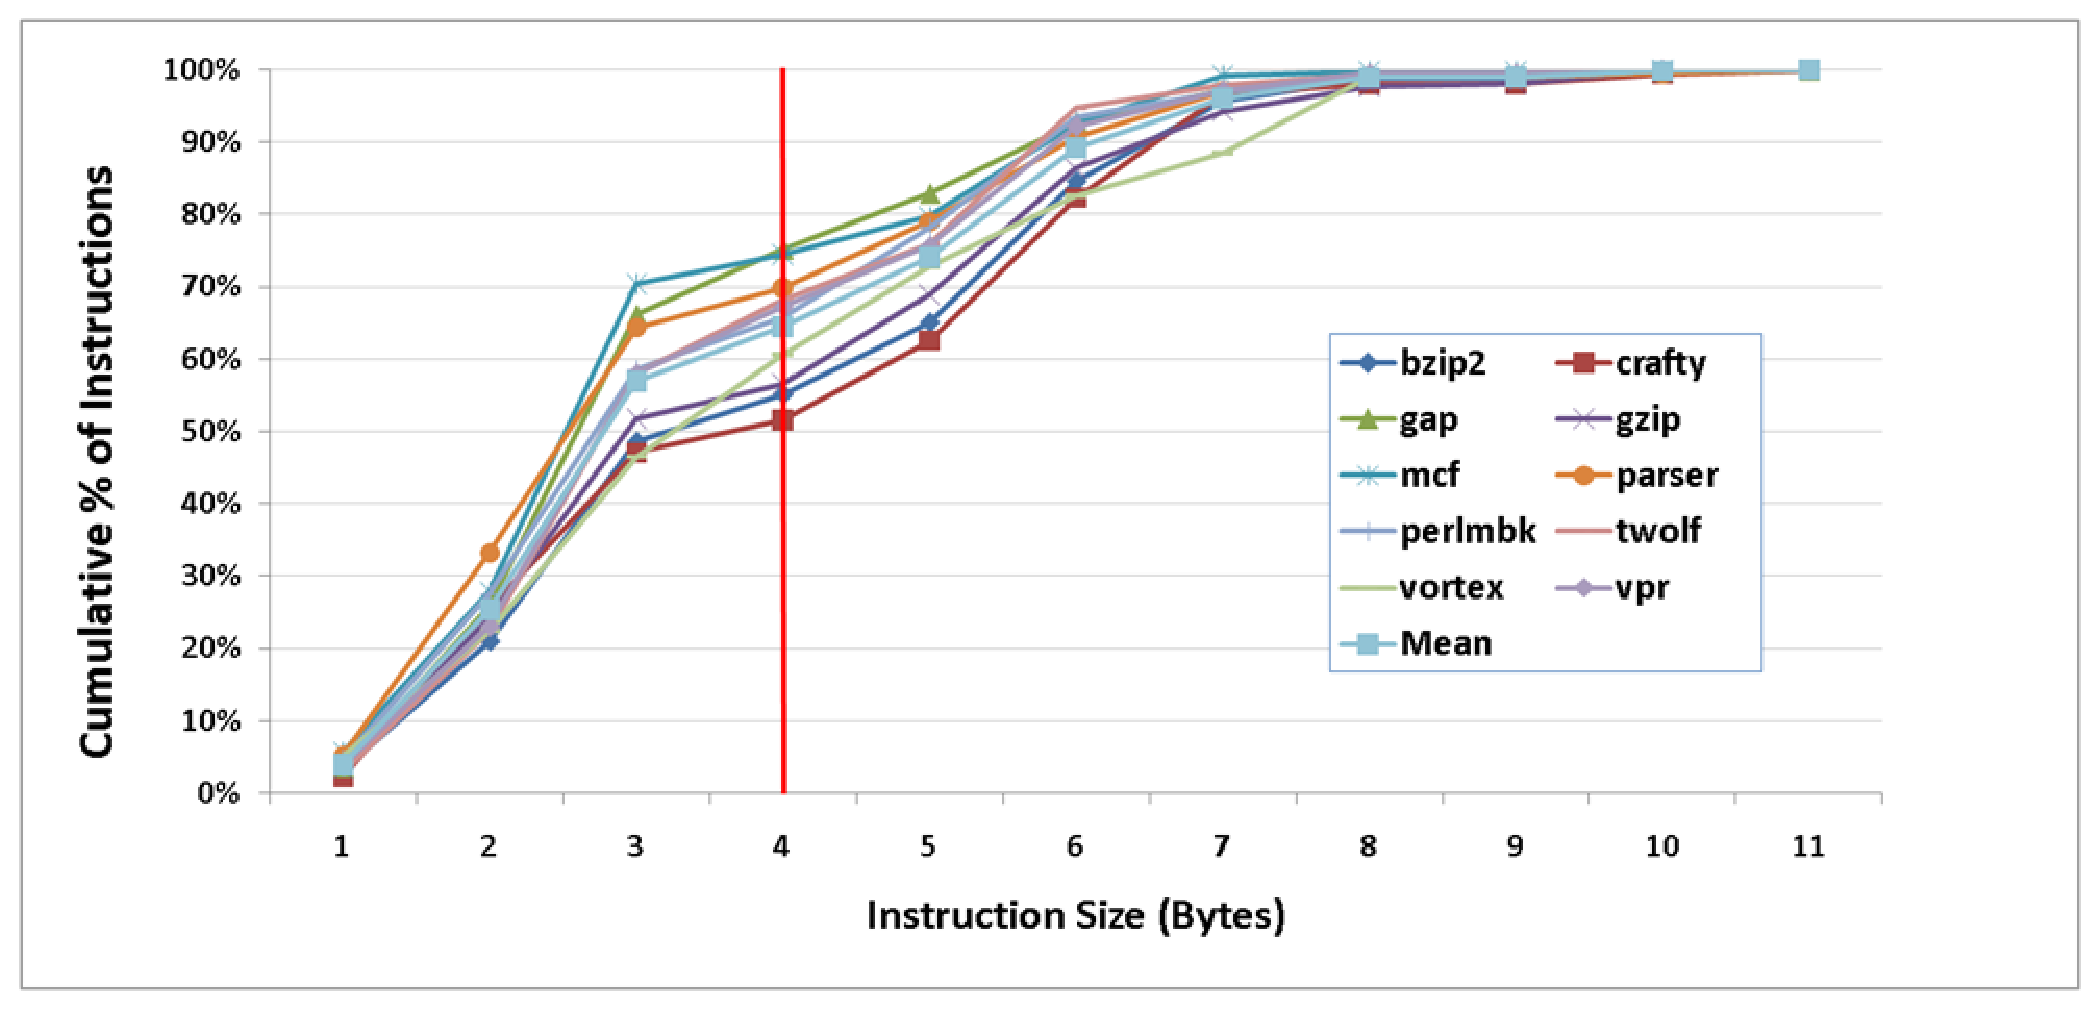
\includegraphics[scale=0.4]{instsize.eps}
\caption{Instruction sizes for a set of benchmarks presented on a cumulative basis.}
\end{figure}

This leaves two options for techniques that can be used to transfer control to
the instrumentation code. Either a technique entirely distinct from the idea of
using a single unconditional branch to execute the control transfer must be used
or somehow the application code must be altered in such a way that it can
accommodate a single large control instruction that is larger than the original
amount of space available at the instrumentation point. One alternative
technique for transferring control flow to an arbitrary point in the
instrumentation code could be to use a series of branches, where the instruction
at the instrumentation point is a small branch that transfers control to a
larger intermediate branch which in turn delivers control to the instrumentation
code. This method is unsatisfactory because the smallest traditional branch
instruction available on the x86 platform is 2 bytes in length, yet there are
instrumentation points with only a single byte available to them. Refer again to
Figure \ref{fig:InstructionSizes}, which shows that an average of 4\% of
instructions use only a single byte. Besides, this technique requires additional
space to be available in close proximity to the instrumentation points since
these smaller 2-byte branches are also short reaching, which is unlikely to be
available since function are often packed tightly within the application text.

Another option is the method proposed by the BIRD project \cite{nanda2006bird},
which is to use a single-byte \begin{it}INT3\end{it} instruction when a larger
traditional branch does not fit at the instrumentation point. This instruction
is functionally perfect for static instrumentation because it consumes only a
single byte and allows us to transfer control to an arbitrary location by using
the exception handling facilities provided by the system. A cursory study was
performed on this scheme from an efficiency standpoint to determine whether it
was worth further investigation. On a small benchmark set, a simple
implementation of using \begin{it}INT3\end{it} only when 5 byte branches do not
fit at the instrumentation point introduces slowdown of at least 100X for even
the simple task of counting the number of executions of each basic block in the
code. As one might expect, this mechanism is unsuitable for efficient
instrumentation because the heavyweight system call conventions are being
invoked on a fairly regular basis to transfer control between the application
and the instrumentation code.

PEBIL uses relocation and reorganization of the code at the function level which
provides is enough space at each instrumentation point to accommodate a 5 byte
jump. Specifically, the steps used by PEBIL to relocate the application's
functions and prepare them for instrumentation are as follows. Figure
\ref{fig:Relocation} shows how this process looks when performed on a trivial
function in order to prepare the function for instrumentation at every basic
block.

\begin{enumerate}
 \item \textit{Function Displacement + Entry Point Linking}
 \item \textit{Branch Conversion}
 \item \textit{Instruction Padding}
 \item \textit{Instrumentation}
\end{enumerate}


\begin{figure}[ht]
\centering
\caption
{The steps taken in order to prepare a function for instrumentation that will
be inserted at every basic block.}
\label{fig:Relocation}
\subfigure[An unmodified application function.]{
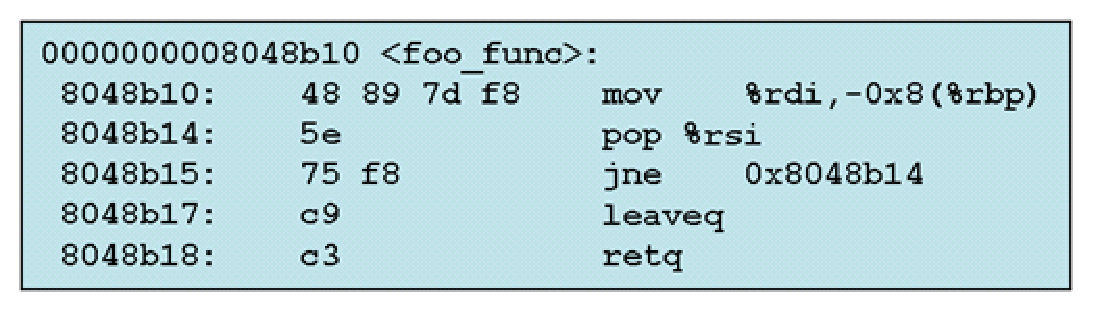
\includegraphics[scale=0.36]{funcp1.eps}
}
\hspace{5mm}
\subfigure[The application function after it has been relocated and the old function entry has been linked to it.]{
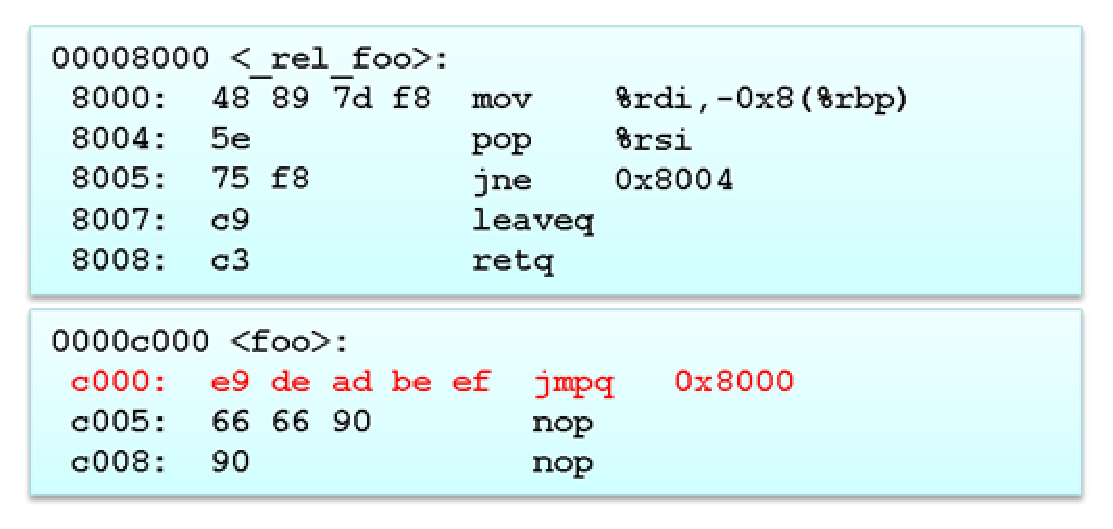
\includegraphics[scale=0.36]{funcp2.eps}
}
\hspace{5mm}
\subfigure[The application function after the branch has been converted to use a 32-bit offset.]{
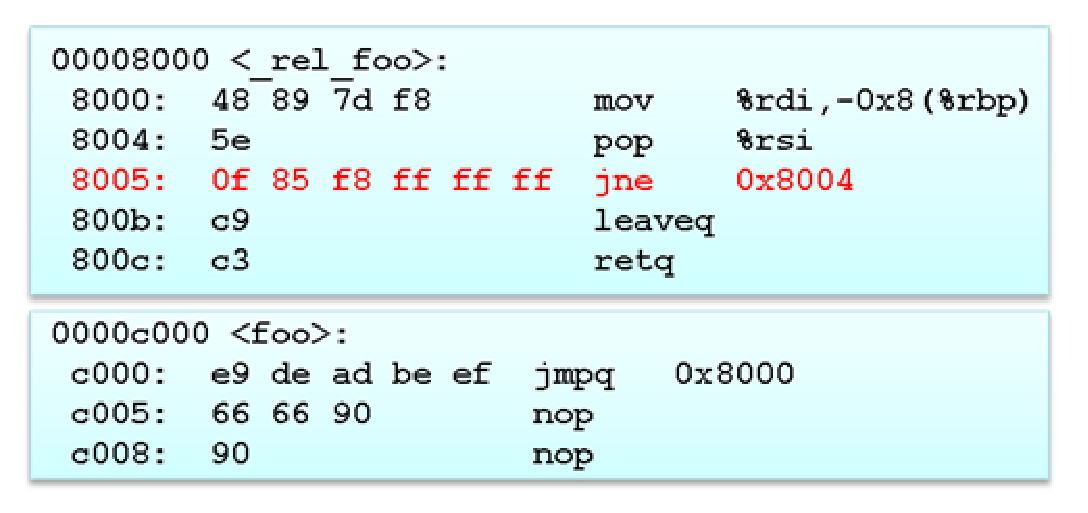
\includegraphics[scale=0.36]{funcp3.eps}
}
\hspace{5mm}
\subfigure[The application function after it has been padded with nop instructions so that each basic block
is large enough to hold a 5 byte jump instruction.]{
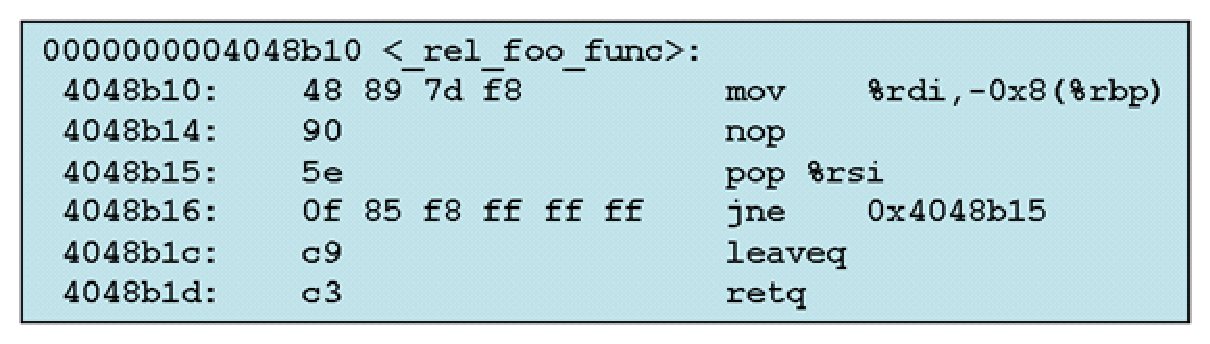
\includegraphics[scale=0.36]{funcp4.eps}
}
\hspace{5mm}
\subfigure[The application function after a single basic block (Basic Block 1) has been instrumented.]{
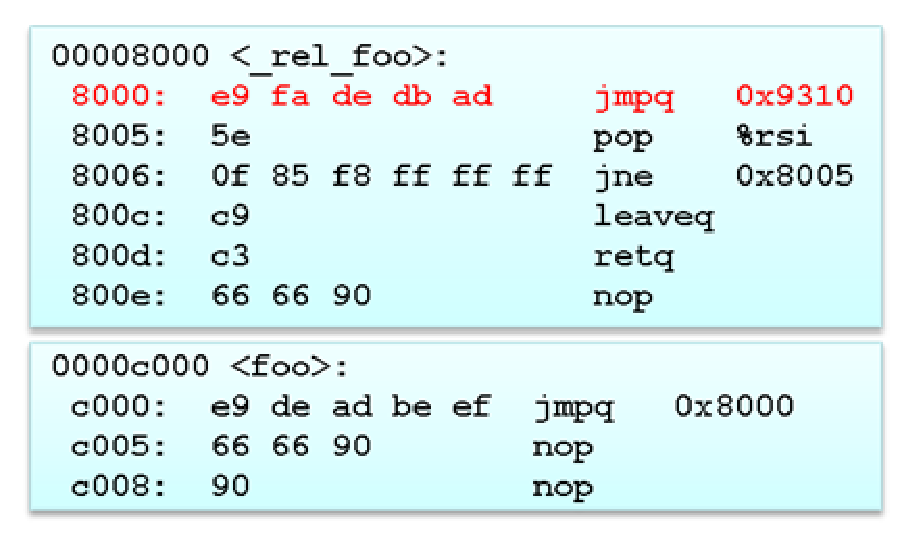
\includegraphics[scale=0.36]{funcp5.eps}
}
\end{figure}


Figure \ref{fig:Relocation}(a) shows a function body prior to any
relocation/instrumentation activities. \textit{Function Displacement + Entry
Point Linking}, shown in Figure \ref{fig:Relocation}(b), relocates the contents
of the entire function to an area of the text section allocated for use by the
instrumentation text. This is done because functions are often packed tightly
together. As a result it is generally not possible to leave a function's entry
point undisturbed and expand its size in a straightforward way without
disturbing the entry point of another nearby function. The original entry point
of the function is then linked to the new location by inserting
an unconditional branch at the original function entry to transfer control to
the displaced function entry. Linking is done in this fashion because most
references to the entry point of a function are in the form of function calls,
which routinely are indirect references (i.e. their value is computed or looked
up at runtime) and are difficult to resolve prior to runtime. \textit{Branch
Conversion}, shown in Figure \ref{fig:Relocation}(c), converts each short branch
in the relocated function to the equivalent 5 byte branch instruction. Since the
code is being reorganized in the next step, which may strain the limits of
smaller 8-bit or 16-bit offsets, all branches are converted to use 32-bit
offsets so that the targets of each branch will still be reachable without the
need to make further changes to the code. Note that there may be some
opportunity here to reduce space by using the smallest branch offset size that
accommodates the branch, but currently a single unified technique is used
to simplify the implementation. Our experiments in Section
\ref{sec:Results} also indicate that the opportunities for improving efficiency
for this technique are minimal. \textit{Instruction Padding}, seen in Figure
\ref{fig:Relocation}(d), pads each instrumentation point, in this case each
basic block, with \begin{it}nop\end{it} instructions so that a 5 byte branch can
be accommodated. \textit{Instrumentation} replaces the instructions at each
instrumentation point with a jump that transfers control to the instrumentation
code, which is shown in Figure \ref{fig:Relocation}(e).

There are several ways that whole function relocation may adversely affect the
performance of the instrumented executable apart from of the overhead that
will be imposed by the instrumentation code. Each function call now
has an extra control interruption associated with it since control must be
passed first to the original function entry point and then to the relocated
function entry point. In addition it is possible that using 32-bit offsets for
every branch rather than some smaller number of bits has an overhead associated
with it. Since the code is being reorganized and expanded, some positive
alignment and size optimizations that the compiler might have made on the
instructions in the function might be destroyed. Finally our technique
introduces extra instructions to be executed in the form of nops.

To quantify the impact of function relocation and the other organizational
changes on application performance, we generated executables in which functions
are relocated, branches are converted to use 32-bit offsets, instruction padding
is applied, yet no instrumentation is introduced. These executables can be used
to measure the overhead of the transformations applied to the executable in
order to prepare it for instrumentation independent of any overhead imposed by
the instrumentation itself. The overhead on a set of ten of the SPECINT 2000
benchmarks never exceeds 6.5\%, with an average overhead of just 1.6\%. Thus the
basic overhead incurred by code relocation and transformation in PEBIL to
accommodate all instrumentation points is well within reason and does not
represent a significant hurdle for efficiency of the instrumented code.

\subsection{Efficient Instrumentation Snippets}

With many instrumentation toolkits, the tasks performed by the instrumentation
tool are accomplished by allowing the user to transfer control from
instrumentation points in the application to instrumentation functions provided
by the user, typically via a shared library or some object code. Since these
instrumentation functions are delivered via a shared library or other object
code, the instrumentation tool developer has the advantage of being able to use
a software development toolchain to write the code in a language that
compiles to the underlying object code. However, the instrumentation function as
a functional mechanism is heavyweight due to the overhead of performing a
function invocation including saving the complete machine state for all
possibles cases that occur in the function. In cases where efficiency is
important, it can be more desirable to insert small sequences of assembly code
to perform a task and only save the small subset of machine state that will be
affected rather than relying entirely on instrumentation functions and the more
costly state preservation that comes with their use.

Most of this state preservation is in the form of register saving and restoring,
but some of it comes in the form of protecting the application call stack from
the instrumentation function. The call stack requires protection from the
instrumentation code during execution because compilers will often optimize leaf
functions in the application by not explicitly creating a stack frame for the
local function data to operate in. This optimization is safe for the application
because during its normal execution a leaf function will never call another
function and thus its wayward stack contents can never be destroyed. In the case
of an instrumented application that calls an instrumentation function from a
leaf, this guarantee no longer holds. Thus, the area above the stack needs to be
protected when an instrumentation function is called from a leaf function.
During the disassembly of a function, PEBIL notes whether it is a leaf function
(i.e. whether it contains any call instructions). Later, during instrumentation,
it automatically protects the stack contents from any instrumentation function
calls made from that function by incrementing the stack pointer by a fixed
amount\footnote{Currently this amount is set to 4 kilobytes, which is large
enough to accommodate the stack usage of all of the leaf functions we have
encountered so far}, which has the effect of giving the leaf function a large
fixed-size stack frame while the instrumentation function is active.

A good example of the efficiency of using instrumentation snippets rather than
instrumentation functions is an instrumentation point at which the desired
outcome for the instrumentation tool is to increment a counter that resides in
memory. In order to accomplish this task with an instrumentation snippet,
control is transferred to the instrumentation point's trampoline which will save
the platform's flags register, update the counter in memory, restore the flags
register, then transfer control back to the application. If instead one used an
instrumentation function, prior to performing the task, the trampoline must save
the flags register, any registers used by the function, and possibly perform
stack protection. It also requires at least 2 more control transfers in order to
enter and exit the instrumentation function. Furthermore these control flow
transfers generally use the call/return paradigm, which in addition to changing
the application's program counter will also store and retrieve information about
the function call site onto the stack, making the use of a snippet a more
efficient choice.

In addition, the use of the instrumentation function is also likely to pollute
the instruction cache more than using a compact instrumentation snippet. For an
instrumentation snippet the application code must contend with the trampoline
code only, whereas using an instrumentation function puts the function code in
contention with the application and the trampoline. Hence, instrumentation
functions tend to be more heavyweight than instrumentation snippets and using
snippets rather than functions whenever possible allows us to gather
\textit{asynchronous} program information more efficiently. Intuitively,
asynchronous information can be thought of as any information that could be
dumped to disk and processed offline. Gao et. al. \cite{gao2005aliter}
demonstrate that using lightweight instrumentation snippets to buffer
information which is later processed by more heavyweight instrumentation
functions in batches is an efficient yet entirely lossless way for
instrumentation tools to process asynchronous program information. The
availability of instrumentation snippets gives tool developers the flexibility
to choose either snippets or functions depending on their performance goals and
software engineering needs.


\section{Results}
\label{sec:Results}

The main design goal of PEBIL is to generate efficient instrumented code. To
investigate the efficiency of instrumented executables created by PEBIL, we ran
several experiments on a selection of benchmarks from the the SPEC CPU2000
Integer benchmark suite comprised of bzip2, crafty, gap, gzip, mcf, parser,
perlmbk, twolf, vortex and vpr. All of the experiments are run on a single core
of a quad-core 2.4GHz IA32 Intel Xeon running Red Hat Linux Enterprise 4.1.2
(Linux kernel 2.6.18). 

The first set of experiments quantifies the overhead of the program relocation
and transformation techniques used by PEBIL as described in Section
\ref{Subsection:Relocation}. Recall that this technique adds an additional
unconditional branch execution to each function call in order to relocate the
function, extends all of the branches in the code to use 32-bit offsets, and
pads each basic block whose size is fewer than 5 bytes with nops so that a 5
byte jump to the instrumentation code can be inserted. These transformations were
performed on our benchmark set so that the code was ready for the insertion of
instrumentation code to measure the overhead caused by relocation and transformation. 

Figure \ref{fig:RelocOverhead} presents the runtime overhead seen in the
instrumentation-ready executables as a percentage of the original application
runtime. The figure shows that the maximum overhead due to these modifications
is 6.5\%, with an average overhead of just 1.6\%. Among a set of popular dynamic
instrumentation toolkits, Pin, DynamoRIO and Valgrind, the lowest overhead for
running the application within the instrumentation tool but performing no
instrumentation is obtained by using DynamoRIO. DynamoRIO has an average of 38\%
overhead and a maximum overhead of 113\% on the SPEC CPU2000 Integer benchmark
set \cite{luk2005pin}. This confirms that the relocation and transformation
method used by PEBIL has a minimal performance impact on the performance of
these benchmarks and thus is a suitable approach as a basis for producing
efficient instrumented code.

\begin{figure}[ht]
\centering
\label{fig:RelocOverhead}
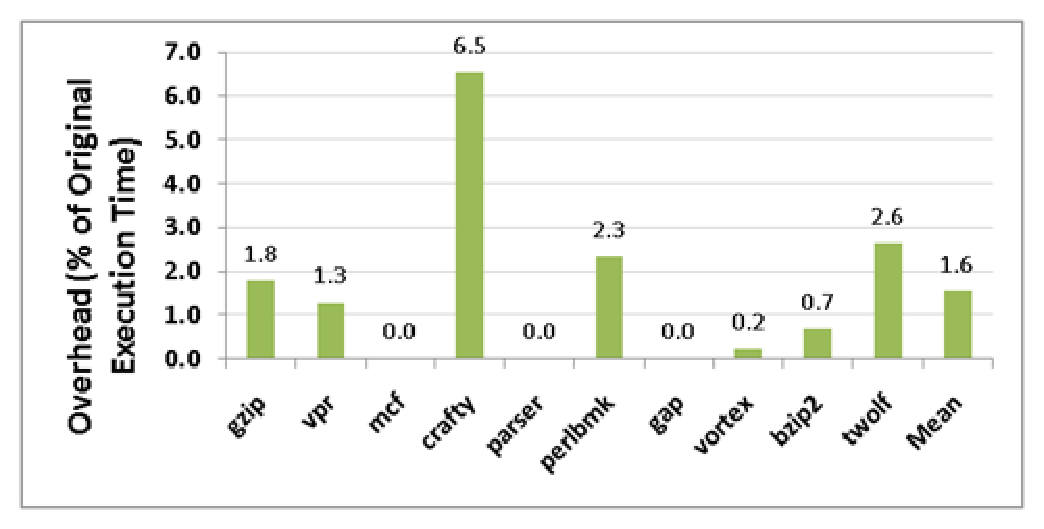
\includegraphics[scale=0.6]{relocperf.eps}
\caption{Application overhead caused by preparing the code for instrumentation but without
any instrumentation inserted.}
\end{figure}

The next set of experiments measure the overhead introduced due to counting the
basic block executions in the application. We use this particular
instrumentation tool because basic block counting is an example of an
instrumentation tool where we would expect PEBIL to generate efficient
instrumented executables since the number of instrumentation points required is
high. Much of the work performed in basic block counting, namely updating a
single counter every time a basic block is encountered, can be done easily using
a fast instrumentation snippet rather than by a full instrumentation function.
The counters embodied in the instrumentation snippets must also be persistent
throughout the entire run of the application, which is more suited to a static
instrumentation approach because the static instrumentation does not utilize any
resources to determine whether instrumentation can be removed. The basic block
counting instrumentation tool was used to produce an instrumented executable for
each program in our benchmark suite, whose runtime was compared to the runtime
of the unmodified original executable. The results of these experiments are
shown in Figure \ref{fig:ToolOverheads}. 

\begin{figure}[ht]
\centering
\label{fig:ToolOverheads}
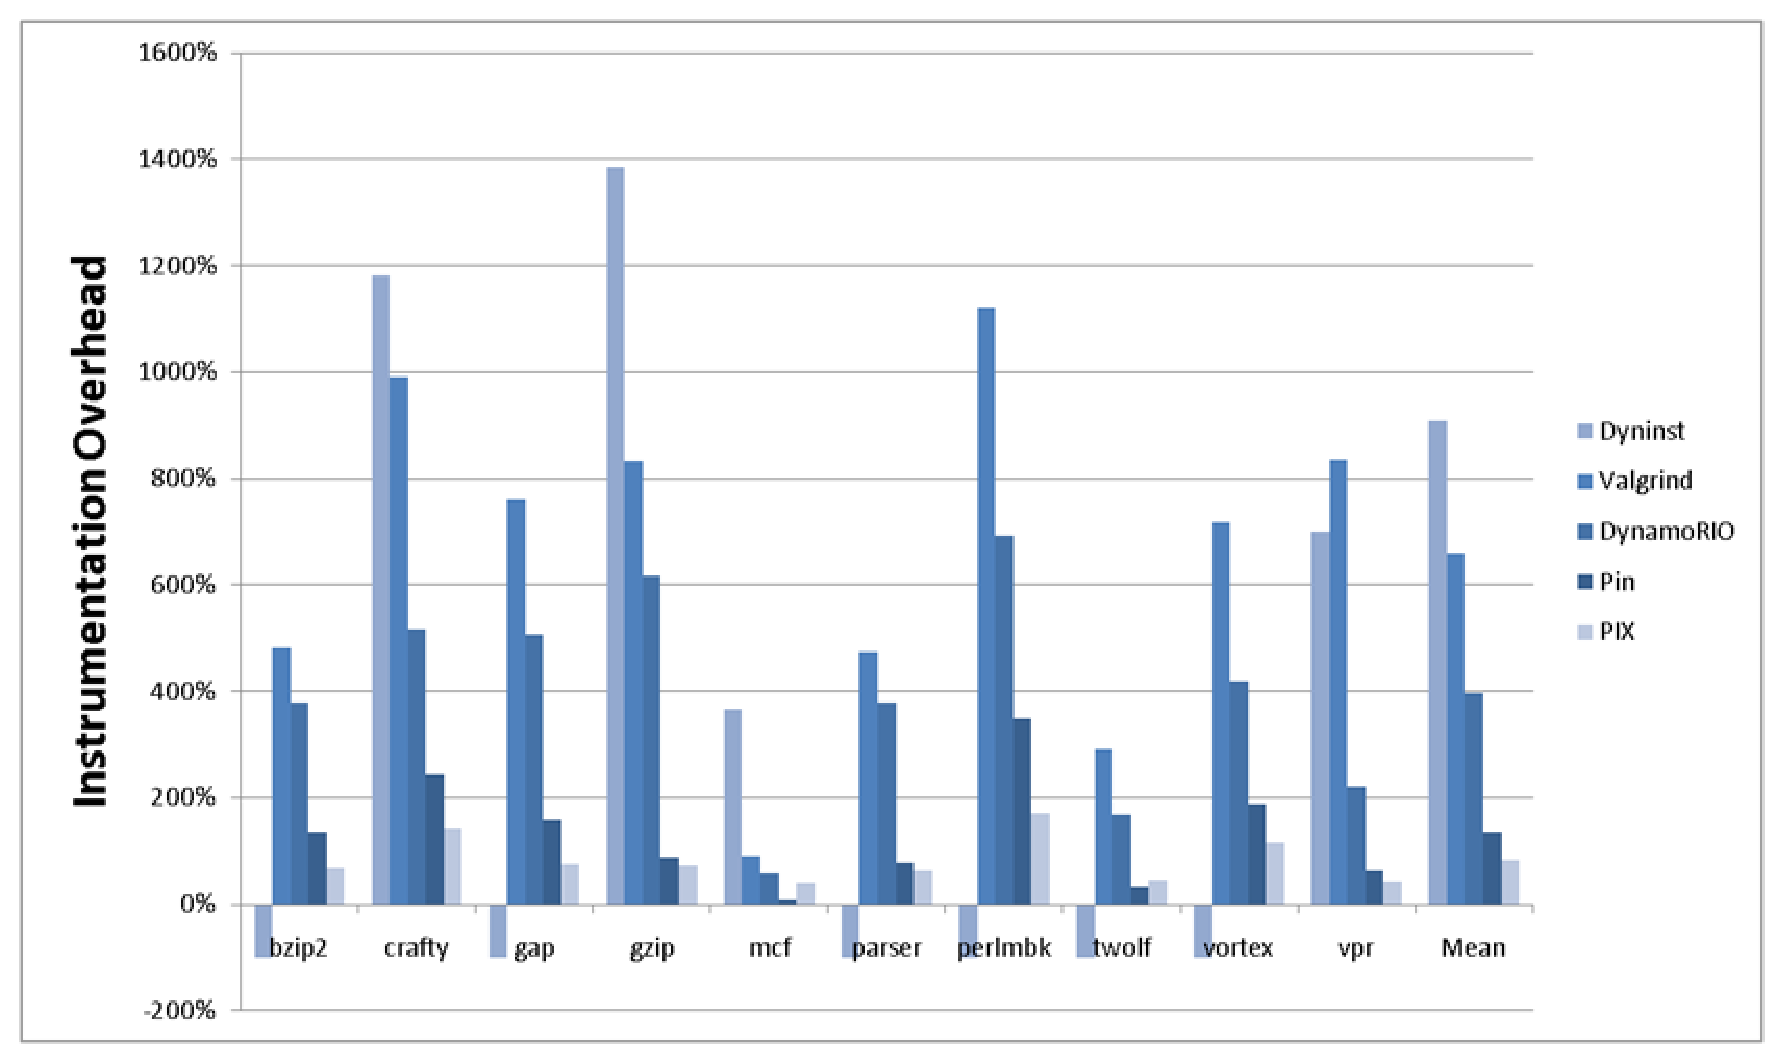
\includegraphics[scale=0.32]{bbcount.eps}
\caption{Performance of several x86 instrumentation tools with basic block counting instrumentation.}
\end{figure}

Figure \ref{fig:ToolOverheads} presents the overhead introduced as a percentage
of the original application runtime. The overhead of PEBIL's basic block counter
ranges from 41\%-170\% for the benchmarks tested with an average overhead of
84\%. More importantly, the figure shows that the overhead introduced by PEBIL
instrumentation is significantly lower than those introduced by the other
instrumentation toolkits available for the x86 platform. The average overhead is
135\% for Pin (ranging from 8\%-350\%), 396\% for DynamoRIO (ranging from
58\%-693\%), 660\% for Valgrind (ranging from 91\%-1120\%), and 1936\% for
Dyninst (ranging from 367\%-7859\%). Our experiments demonstrate that
executables instrumented by PEBIL run an average of 51\% faster than Pin, which
is the next most efficient instrumentation toolkit for basic block counting.
Furthermore, Pin uses a variety of optimizations such as tracking eflags bit
liveness \cite{luk2005pin} that are currently unincorporated into PEBIL. We plan
to incorporate more optimizations into PEBIL in the future (see Section
\ref{sec:Future}) including several optimizations already in use by Pin, which
should further improve the efficiency of the instrumented executables generated
by PEBIL.



\section{Future Work}
\label{sec:Future}

Despite the success in terms of efficiency, there are several additional techniques
that might make the instrumented code even more efficient in PIX. Because PIX relocates
the text to yeild extra space for the manipulation of the application functions, 
rather than inserting just a branch
that transfers control to the instrumentation code we have the opportunity to inline
the instrumentation code itsself
in order to reduce or eliminate the control interruptions  that otherwise must be taken 
when inserting the instrumentation code.

Currently PIX saves all general purpose registers around each function call and allows the
tool developer to state which registers are saved around instrumentation snippets. For even more efficient instrumentation
snippets, we could automatically detect which registers are killed by the instrumentation code and which are live at the entry point
of the instrumentation code, and automatically save only the ones that are alive. Similarly, we could perform register 
analysis in order to identify the instrumentation points where the machine state doesn't need to be saved around instrumentation functions. 

Finally, similar to Pin, we could perform liveness on the bits of the eflags/rflags register to determine whether the flag registers need to be saved and
restored at each instrumentation point. Optimizations that help PIX avoid saving and restoring state at each instrumentation point 
have the potential to further the overhead associated with instrumentation and we beleive 
that they will further the goal of generating efficient instrumented code with PIX.




ATOM [CITE] was one of the first and has remained one of
the more popular static binary instrumentation tools
available. ATOM works in a way that is very similar to
PMaCinst; instrumentation is performed on the compiled
binary prior to runtime, meaning that any overhead due to
code analysis and code generation is incurred outside of
the instrumented application’s runtime. Unfortunately,
ATOM is available only for the Alpha platform. Since this
processor is not being produced anymore, ATOM is no
longer viable as a long-term solution for those who wish to
perform static, efficient instrumentation on a RISC-based
platform. 

Pin[CITE] is a dynamic binary instrumentation tool that
uses a JIT-based (Just In Time compilation) approach to
instrumentation. This approach entails running the
application on top of Pin, while Pin intercepts the
application at a natural control flow interruption in the
program to perform instrumentation on the next part of the
program. For efficiency, Pin does many things including
caching these instrumented sequences of code to allow for
re-use and chaining instrumented sequences of code
together to avoid tool intervention.

Dyninst[CITE] is another popular dynamic
instrumentation tool that uses a technique called codepatching
to perform instrumentation. Similar in concept to
what is done in PMaCinst, this technique replaces an
instruction from the application with a jump instruction
(which they call a trampoline) to the function call stub and
instrumentation code. The key difference between
PIX and Dyninst is that Dyninst performs all codepatching
at runtime instead of prior to runtime. This has
several advantages, including the ability to insert, remove
and customize instrumentation during runtime. But
performing modification to the program at runtime also
may have a significant performance disadvantage, resulting in
inefficient execution of the instrumented application.

DynamoRIO

Valgrind


\section{Conclusions}


\bibliography{x86inst}
\bibliographystyle{unsrt}

\end{document}

